\section{Analyse}
Nachfolgend werden alle kritischen Elemente der SDA Lösung analysiert. Dazu gehören beispielsweise Dienste, wie die LISP Datenbank, Radius, SGT Access List. und 

Das Ziel ist die komplette Analyse der SDA Lösung und die Identifizierung der kritischen Elemente der Verfügbarkeit (LISP Database, Radius, SGT Access-list etc.) und der Network Services (NTP, DNS, Lizenzen etc.).

\subsection{Architektur}
Unsere Architektur der Lab Umgebung, welche in der Studienarbeit erarbeitet und nun in der Bachelorarbeit noch erweitert wurde, sieht zur Zeit wie folgend aus:

\begin{figure}[H]
	\centering
	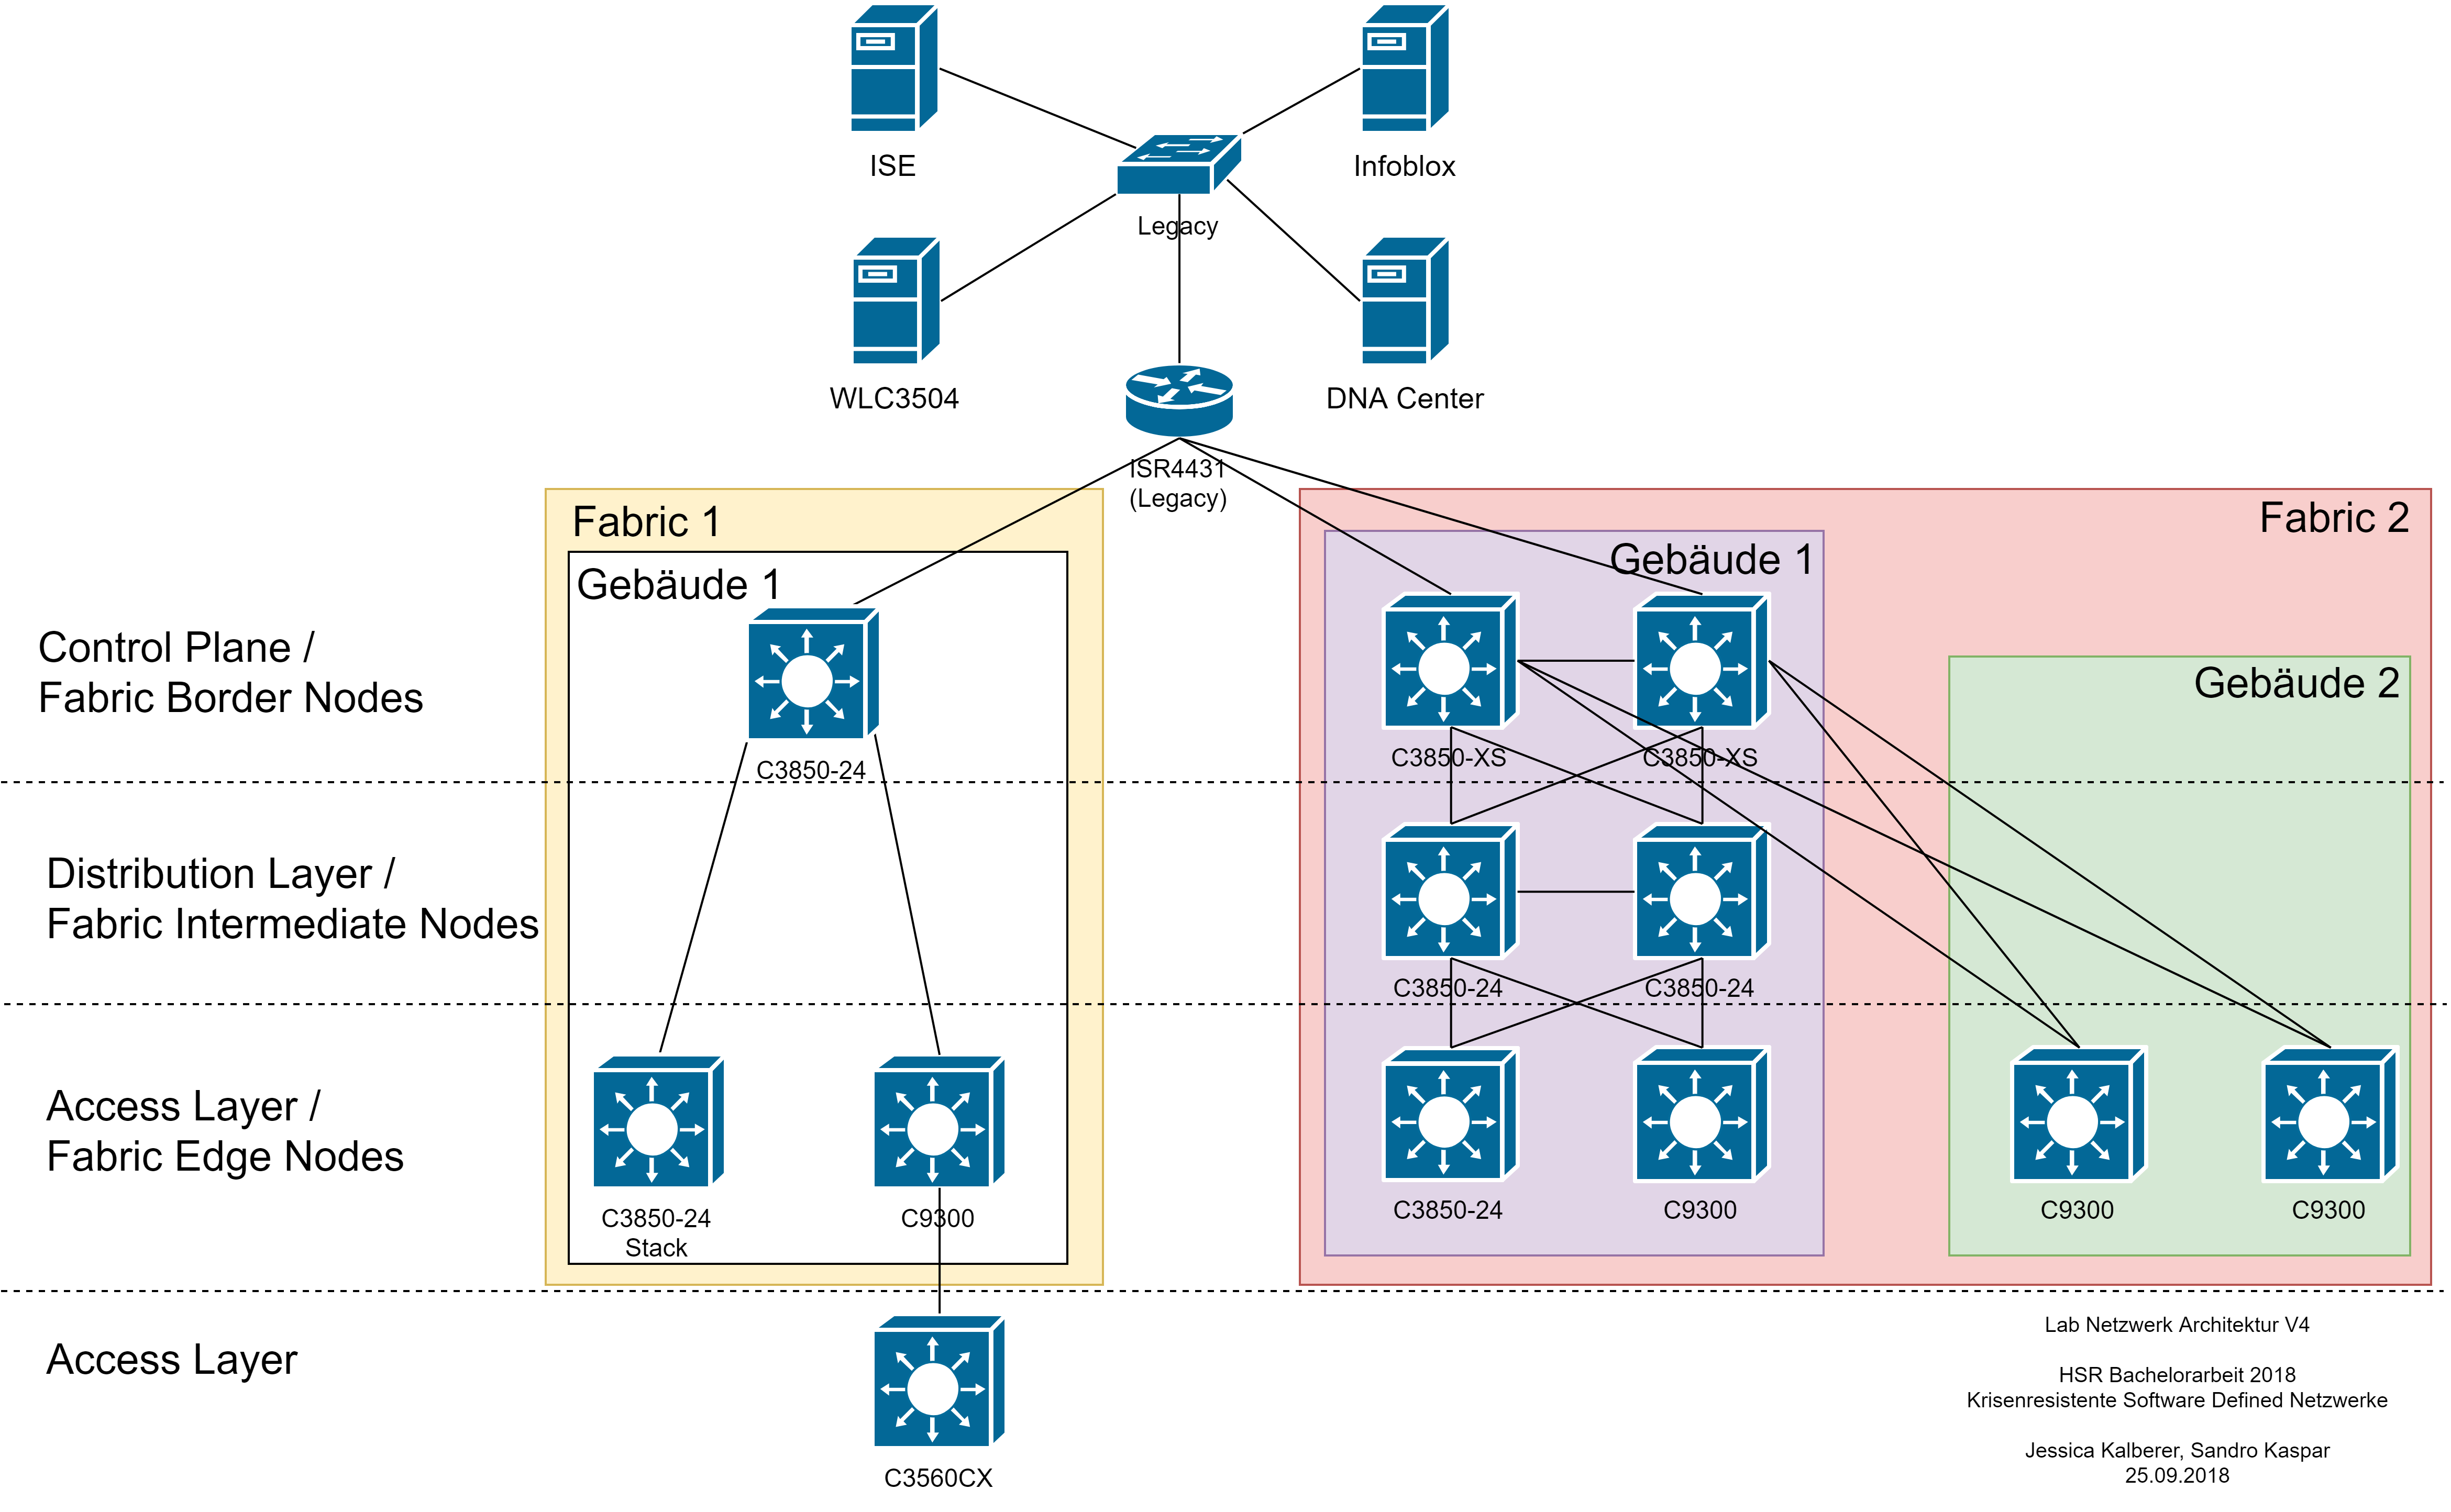
\includegraphics[width=1\linewidth]{img/Architecture/LabNetworkArchitecture-25-09}
	\caption{Architektur}
	\label{fig:Architektur}
\end{figure}

Die Analyse wird auf dieser Architektur aufbauen und die von der FUB gegebenen Grössenordnung berücksichtigen.